%-*- coding: utf-8 -*-
\documentclass{beamer}

\usepackage[frenchb]{babel}
\usepackage[T1]{fontenc}
\usepackage[utf8]{inputenc}
\graphicspath{{images/}}
\usepackage{csquotes}
\usepackage{tocvsec2}
\maxtocdepth{section}
\usetheme{Warsaw}
\setbeamertemplate{headline}{} % Supprime la zone de menu en haut (prend trop de place !)

\title{Projet Arrosage}
%\subtitle{Sous-titre}
\author{S HADJOUTRIOS, J GARCIA, E IGUAL, JF BENITEZ} % Si on met les noms en majuscules, il y en a un de tronqué en bas dans le pied de page.
\institute{CNAM}
\date{21/02/2018}

\logo{
\includegraphics[height=10mm]{ipst-cnam.png}}
\setbeamertemplate{background canvas}{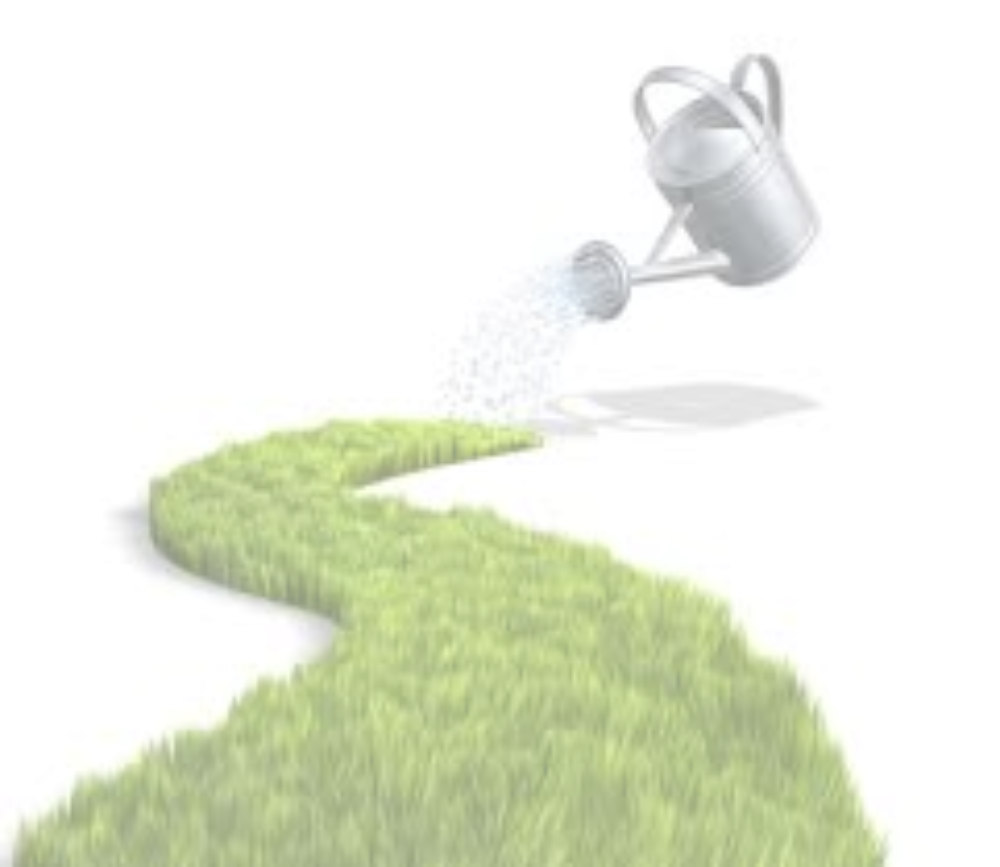
\includegraphics[width=\paperwidth,height=\paperheight]{arrosage.png}} % Width pour la largeur, height pour la hauteur de l'image

\begin{document}
\begin{frame}[plain]
  \titlepage
\end{frame}

\begin{frame}
  \frametitle{Sommaire}
  \tableofcontents
\end{frame}

\section{Finalité}
\begin{frame}[label=finalite]
  \frametitle{Finalité}
  \rightskip=0pt\leftskip=0pt
  La finalité du système d'arrosage est ...
\end{frame}

\subsection{Missions}
\begin{frame}[label=missions]
  \frametitle{Missions}
  \rightskip=0pt\leftskip=0pt
  Les missions du système d'arrosage sont ...
\end{frame}

\subsection{Fonctions de services}
\begin{frame}[label=fonctionsdeservices]
  \frametitle{Fonctions de services}
  \rightskip=0pt\leftskip=0pt
  Les fonctions de services du système d'arrosage sont ...
\end{frame}

\end{document}
